\section{The Hard Parts of Software Architecture}
The following section contains the content of a guest lecture about the book: \href{https://www.oreilly.com/library/view/software-architecture-the/9781492086888/}{Software Architecture: The Hard Parts}.

\subsection{Service Granularity}
\begin{minipage}[t]{0.5\textwidth}
	\textbf{Granularity Disintegrators}
	Provide guidance and justification for when to break a service into smaller pieces.
	\begin{itemize}
		\item Service scope and function: Is the service doing too many unrelated things?
		\item Code volatility: Are changes isolated to only one part of the service?
		\item Scalability and throughput: Do parts of the service need to scale differently?
		\item Fault tolerance: Are there errors that cause critical functions to fail within the service?
		\item Security: Do some parts of the service need higher security levels than others?
		\item Extensibility: Is the service always expanding to add new contexts?
	\end{itemize}
\end{minipage}
\begin{minipage}[t]{0.5\textwidth}
	\textbf{Granularity Integrators}
	Provide guidance and justification for putting services back together (or not breaking apart a service in the first place).
	\begin{itemize}
		\item Database transactions: Is an ACID transaction required between separate services?
		\item Workflow and choreography: Do services need to talk to one another?
		\item Shared code: Do services need to share code among one another?
		\item Database relationships: Although a service can be broken apart, can the data it uses be broken apart as well?
	\end{itemize}
\end{minipage}

\paragraph{Tradeoff Analysis} 
\begin{enumerate}
	\item Find what parts are coupled together
	\item Analyze how they are coupled to one another
	\item Assess the tradeoffs by determine the impact of change to interdependent system
\end{enumerate}

\begin{figure}[H]
  \center
  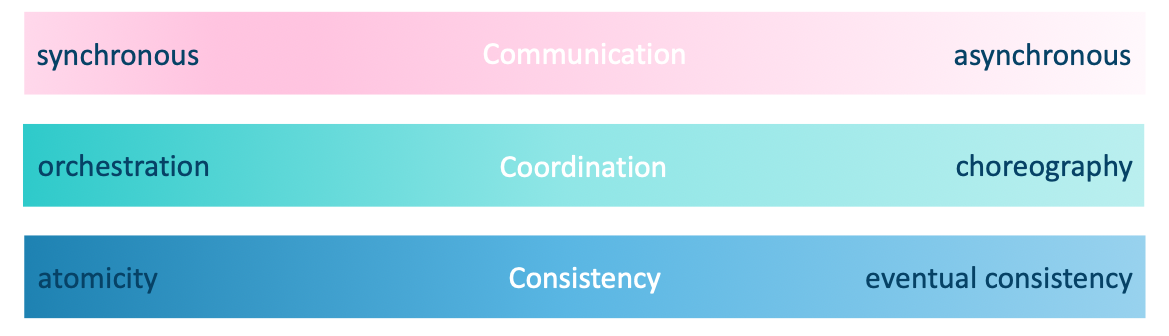
\includegraphics[width=0.75\textwidth]{tradeoffanalysis}
  \caption{Tradeoff Analysis}
\end{figure}

\subsubsection{Communication}

\begin{minipage}[t]{0.5\textwidth}
	\textbf{Synchronous Tradeoffs}
	\begin{itemize}
		\item - Perfomance impact on highly interactive systems
		\item - Create dynamic entanglements
		\item - Creates limitations in distributed architectures
		\item + Easy to model transactional behaviour
		\item + Mimics non-distributed method calls
		\item + Easier to implement
	\end{itemize}
\end{minipage}
\begin{minipage}[t]{0.5\textwidth}
	\textbf{Asynchronous Tradeoffs}
	\begin{itemize}
		\item - Complex to build and debug
		\item - Presents difficulties for transactional behaviours
		\item - Error handling
		\item + Allows highly decoupled systems
		\item + Common performance tuning technique
		\item + High performance and scale
	\end{itemize}
\end{minipage}

\subsubsection{Orchestration}

\begin{minipage}[t]{0.5\textwidth}
	\textbf{Orchestration Tradeoffs}
	\begin{itemize}
		\item - Responsiveness
		\item - Fault tolerance
		\item - Scalability
		\item - Service coupling
		\item + Centralised workflow
		\item + Error handling
		\item + Recoverability
		\item + State management
	\end{itemize}
\end{minipage}
\begin{minipage}[t]{0.5\textwidth}
	\textbf{Choreography Tradeoffs}
	\begin{itemize}
		\item - Distributed workflow
		\item - State management
		\item - Error handling
		\item - Recoverability
		\item + Responsiveness
		\item + Fault Tolerance
		\item + Scalability
		\item + Service decoupling
	\end{itemize}
\end{minipage}

\begin{figure}[H]
  \center
  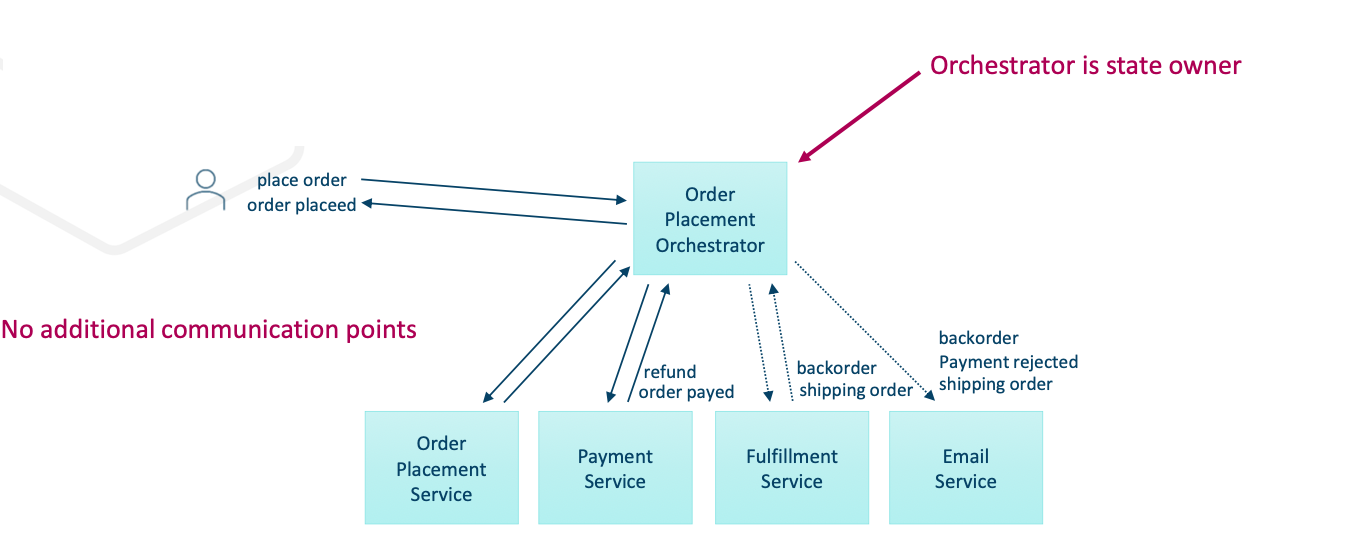
\includegraphics[width=\textwidth]{orchestration.png}
  \caption{Ochestration Workflow}
\end{figure}


\begin{figure}[H]
  \center
  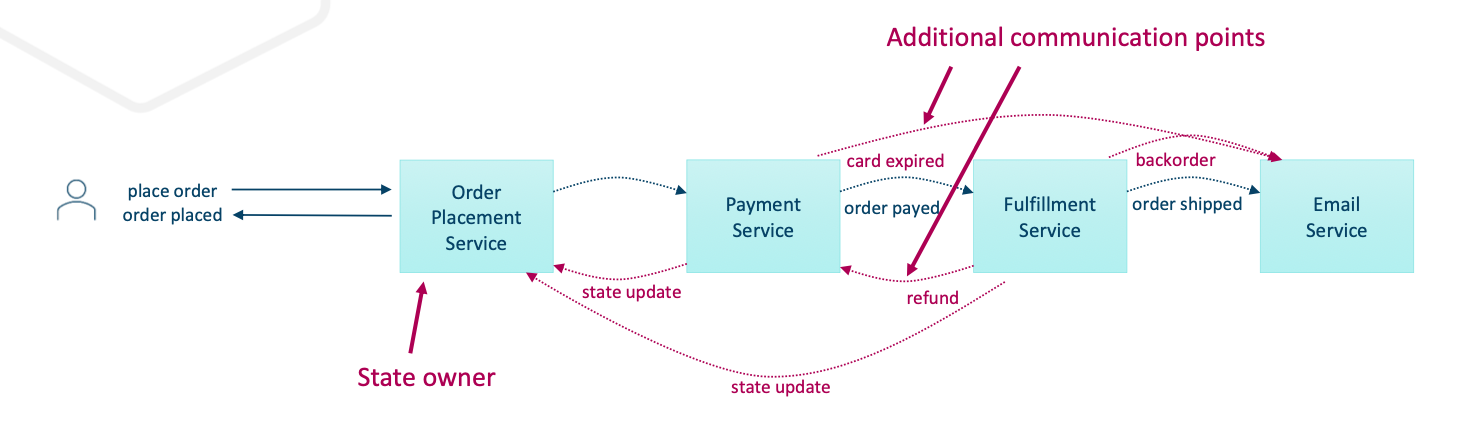
\includegraphics[width=\textwidth]{choreography.png}
  \caption{Choreography Workflow}
\end{figure}

